%!TEX root = ../CallenThermo.tex

\chapter{可逆过程和最大功定理}\label{chap4}

\section{可能和不可能的过程}\label{sec4.1}

一名工程师常会需要通过设计一个装置来完成某个任务——例如让一个电梯升到高楼上。因此他就得弄出一个联动装置,或者“引擎”,来可控的将能量从火炉里转移到电梯上;{\it 如果}火炉里的热量通过数个活塞、杠杆和凸轮转换成了电梯上升所需要的能量。但谋事在人,成事由“天”(例如,物理定律)%
\mpar{原文为 "But 'nature'(i.e. the law of physics) exercise the crucial decision"}%
——这件事到底是能办成呢,还是设备干脆就停着不动,没有热量从火炉里出来,电梯也没上升一丝一毫。结果得取决于两点。其一是引擎得要满足力学定律(自然包括能量守恒),其二,这个过程必须最大化地使熵增加。\mpar{此处存疑,热力学过程只需满足熵增即可,略微偏离平衡区的线性系统才存在有最大熵产生定理。}

专利局里充满了各路在逻辑上无可挑剔的(如果A发生那么B一定发生)失败发明——这些天才般的设计满足所有力学定律,但依旧固执的停在那儿,默默地拒绝熵的减小。其他的一些能动起来,但会产生一些意料之外的结果,比发明者预料中更有效的使熵增加。

如果,虽然如此,这个网络被在保证总能量不变的前提下最大可行的增加总的熵,那么将不会有什么基本定律来否决掉这样一个恰当的过程的存在。尽管实现这样适当的引擎可能需要相当的天才成分,但它起码在原则上来讲是可行的。

\begin{example}\label{eg4.1}
一个约束系统具有确定摩尔数和体积,则其不能对外界做功。另外,这个系统的热容是常数$C$。则这个系统的基本方程是$S=S_0+C\ln(U/U_0)$,其中$U=CT$。\\
两个具有相同热容量的此类系统,初态分别具有温度$T_{10}$和$T_{20}$,其中$T_{10}<T_{20}$。一个用于升降电梯的引擎(即对一个纯力学系统做功),从这两个热力学系统中获取能量。它们最大能获得多少功?\\
{\bf 求解:}\\
这两个热力学系统最终会达到相同的温度$T_f$。其能量的总改变量为
\[
\Delta U = 2CT_f-C(T_{10}+T_{20})
\]
而力学系统(“电梯”)所获得的功为$W=-\Delta U$,即
\[
W = C(T_{10}+T_{20}-2T_f)
\]
熵的总改变量为两个热力学系统的改变量之和,为
\[
\Delta S = C\ln\frac{T_f}{T_{10}} + C\ln\frac{T_f}{T_{20}} = 2C\ln\frac{T_f}{\sqrt{T_{10}T_{20}}}
\]
为了使$W$最大,我们自然希望$T_f$最小(从第二式容易看出),根据第三式我们知道这意味着要使$\Delta S$取极小。而$\Delta S$最小就只能是零了,对应着一个可逆过程。这样最优的引擎能得到
\[
T_f = \sqrt{T_{10}T_{20}}
\]
和
\[
W = C(T_{10}+T_{20}-2\sqrt{T_{10}T_{20}})
\]
\end{example}

作为补充,我们需要注意到假设两个热力学系统最后到达一个相同的温度是不必要的;$W$可以分别对$T_{1f}$和$T_{2f}$作优化,最后能得到同样的结果。对于末温相同这个简化假设,我们可以用自洽性来论证:如果末温不同,那么我们可以通过这个办法来继续获取更多的能量。

\begin{example}
例\ref{eg4.1}的一个有趣的变体是三物体(每一个都是例\ref{eg4.1}中描述的类型,有$U=CT$)初始温度分别为\SI{300}{\kelvin}、\SI{350}{\kelvin}、\SI{400}{\kelvin}。其需求是尽可能高的提高{\it 一个}物体的温度,而不论其他两个物体怎么样(并且不改变任何外部系统的状态)。那么这里一个物体最高能到多高温度?\\
{\bf 求解:}\\
将三个初始温度用$T_1$,$T_2$,$T_3$标记,单位取作\SI{100}{\kelvin}($T_1=3$,$T_2=3.5$以及$T_3=4$)。类似的,令单个物体能达到的最高温度记做$T_h$。可以推断剩下两个物体的末温{\it 都}是$T_c$(否则,我们可以用例\ref{eg4.1}的办法来对外做功,然后将功转换为热物体上的热)。能量守恒要求
\[
T_h + 2T_c = T_1 + T_2 + T_3 = 10.5
\]
总的熵增为
\[
\Delta S = C\ln\frac{T_c^2T_h}{T_1T_2T_3}
\]
熵增为正要求
\[
T_c^2T_h \ge T_1T_2T_3 \quad (=42)
\]
利用能量守恒式消去$T_c$
\[
(5.25-\frac{T_h}{2})^2T_h\ge 42
\]
方程左端对$T_h$作图。绘图范围从$0$到$10.5$,上界是为了保证$T_c$为正。图像表明使纵坐标大于$42$的最大$T_h$值是
\[
T_h = 4.095 \quad(\text{或}T_h = \SI{409.5}{\kelvin})
\]
这个值使不等式取等,即对应可逆过程。
\end{example}
\begin{figure}
\centering
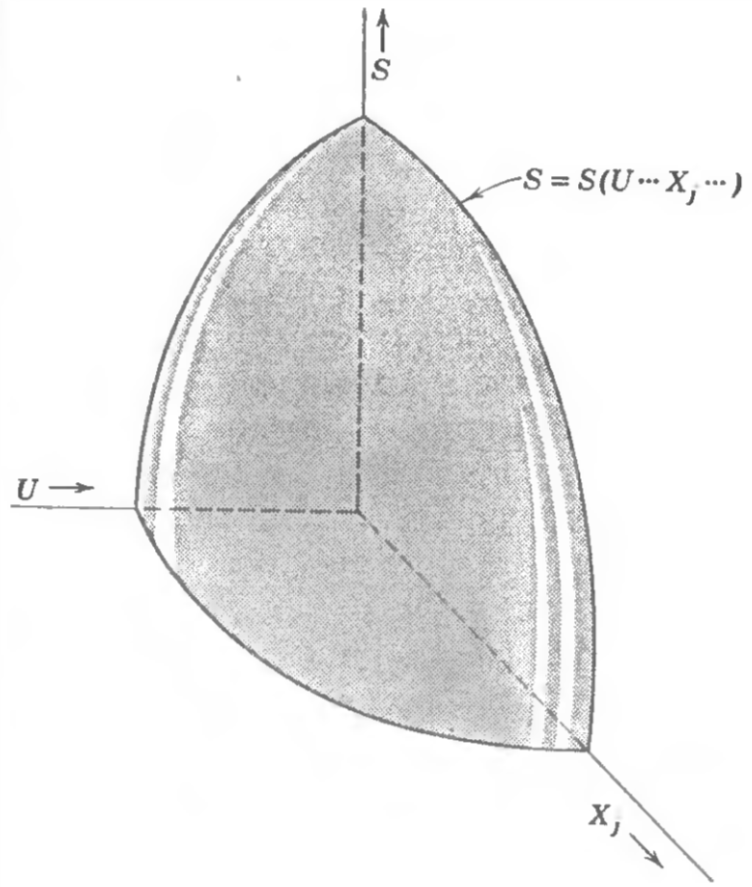
\includegraphics[width=\textwidth]{Pictures/fig4.1.png}
\end{figure}

这道题的另一个解法见习题4.6-7。

\subsection*{习题}
\begin{itemize}
\item[4.1-1.] 一摩尔单原子理想气体和一摩尔$c=3/2$的理想 van der Waals 流体(\ref{sec3.5}节)分别装在体积为$v_1$和$v_2$的容器里。理想气体的温度为$T_1$而 van der Waals 流体是$T_2$。我们希望将理想气体的温度变成$T_2$而保持总的能量不变。那么 van der Waals 流体的末温是多少?各参数($T_1,T_2,a,b,v_1,v_2$)之间需要满足什么关系才能实现这样一个温度转换(总是假定在过程中外界不发生改变)?
\item[4.1-2.] 一个橡胶带(\ref{sec3.7}节)初始温度为$T_B$,长度为$L_{B}$。一摩尔单原子理想气体初温为$T_G$,体积为$V_G$。理想气体经历一个定容升温过程达到温度$T_G'$。其所需要的能量全都从橡胶带中获得。那么橡胶带的长度是否需要改变?如果是的话,改变多少?
\begin{flushright}
{\it 答案:}\\
若$l=L_B-L_0$,
\[
l^2-(l')^2\ge 2b^{-1}cL_0(L_1-L_0)\ln\left(1-\frac{3R}{2RL_0}\frac{T_G'-T_G}{T_B}\right)+3Rb^{-1}(L_1-L_0)\ln(T_G'/T_G)
\]
\end{flushright}
\item[4.1-3.] 假设例\ref{eg4.1}中的两个系统热容具有形式$C(T)=DT^n$,其中$n>0$:\\
\begin{enumerate}
\item 证明这样的系统内能$U=U_0+DT^{n+1}/(n+1)$以及熵$S=S_0+DT^n/n$。系统的基本方程是什么?
\item 如果其初始温度分别为$T_{10}$和$T_{20}$,最大可输出功为多少(两系统最后处于相同温度)?
\end{enumerate}
\begin{flushright}
{\it 答案:}\\
对于$n=2$:
\[
W=\frac{D}{3}\left[T_{10}^3+T_{20}^3-\frac{1}{\sqrt{2}}(T_{10}^2+T_{20}^2)^{3/2}\right]
\]
\end{flushright}
\end{itemize}